
\subsection{Example Scenario of Smart Home}
\begin{figure}
	% \setlength{\belowcaptionskip}{0.1cm}
	\centering
%	\includegraphics[width=0.9\textwidth]{Graph/scenario.png}
    \includegraphics[width=0.9\textwidth]{scenario.png}
	\caption{Example Scenario of Smart Home}
	\label{fig:scenario}
\end{figure}

In this section, we use a scenario shown in Figure~\ref{fig:scenario} to describe the challenges of developing smart home services and the approach used in this article. Scenario includes three locations, which are the sitting room, bedroom and a balcony. Each location sets different intelligent devices, as shown in table 1. For example, the sitting room set air conditioner, smart fan, smart light, PM2.5 Monitor and air purifiers and other device. Scenario include four types of environment status, temperature, humidity, brightness and PM2.5. According to different types of environment condition, intelligent devices can provide monitor, increase, reduce, assign and other services, as shown in table 2. For example, air conditioner can provide temperature monitoring, improvement, reduction and assignment services, air purifier can provide PM2.5 reduction services.

\begin{table}[htbp]
	\caption{Smart Devices in Each Locations}
	\centering  %????
	\label{table1}  % ?????????
	\renewcommand\arraystretch{1.5}  %???????1.5?
	\begin{tabular}{p{3.5cm} p{2.5cm}<{\centering} p{2cm}<{\centering} p{2cm}<{\centering}}  %???????
    \toprule[1.5pt]
	 & Sitting Room & Bedroom & Balcony \\
	\midrule[1.5pt]

	Air Conditioner & 1 & 1 & -\\

	Smart Fan       & 1 & 1 & -\\

	Smart Light     & 1 & 1 & -\\

	PM2.5 Monitor   & 1 & - & -\\

	Air Purifier    & 1 & - & -\\

	Flower Monitor  & - & - & 1\\

	Smart Water Pump& - & - & 1\\

	Smart LED       & - & - & 1\\
	\bottomrule[1.5pt]
	\end{tabular}
\end{table}

\begin{table}[htbp] %????????
	\centering  %????
	\caption{Services Provided by Each Smart Devices}
	\label{table2}
	\renewcommand\arraystretch{1.5}  %???????1.5?
	\begin{tabular}{p{3cm} p{2cm}<{\centering} p{2cm}<{\centering} p{2cm}<{\centering} p{2cm}<{\centering}}  %???????
		
		\toprule[1.5pt]
		& Temperature & Humidity & Brightness & Particulate Matter 2.5 \\
		\midrule[1.5pt]
		
		Air Conditioner & Monitor/Increase/Reduce/Assign & - & - & -\\
		
		Smart Fan       & Monitor/Increase/Reduce/Assign & - & - & -\\
		
		Smart Light     & - & - & Monitor/Increase/Assign & -\\
		
		PM2.5 Monitor   & - & - & - & Monitor\\
		
		Air Purifier    & - & - & - & Reduce\\
		
		Flower Monitor  & - & Monitor & Monitor &\\
		
		Smart Water Pump& - & Increase & - & -\\
		
		Smart LED       & - & - & Increase/Assign & -\\
		\bottomrule[1.5pt]
	\end{tabular}
\end{table}


\begin{table}[htbp]
	\centering  %????
	\caption{Users' Locations and Requirements}
	\label{table3}
	\renewcommand\arraystretch{1.5}  %???????1.5?
	\begin{tabular}{p{2cm}<{\centering} p{2cm}<{\centering} p{2cm}<{\centering} p{2.5cm}<{\centering} p{2cm}<{\centering} p{2cm}<{\centering}}  %???????
		\toprule[1.5pt]
		& Jack & Ken & Sansevieria & Cactus & Lily\\
		& (moving) & (moving) & (sitting room) & (balcony) & (balcony)\\
		
		\midrule[1.5pt]
		
		Temperature & [19$^\circ$C, 26$^\circ$C] & [22$^\circ$C, 26$^\circ$C] & [10$^\circ$C, 35$^\circ$C] & - & -\\ %??^?????\circ????
		
		Humidity    & - & - & - & $>20\%$ & $>60\%$ \\
		
		Brightness  & $>20\%$ & $>20\%$ & $>20\%$ & $>80\%$ & $>70\%$ \\
		
		PM2.5       & $<35\mu g/m^3$ & $<35\mu g/m^3$ & - & - & -\\ %$\mu$
		
		\bottomrule[1.5pt]
	\end{tabular}
\end{table}

The requirements of each user in the scenario are shown in Table~\ref{table3}. User Jack wants indoor temperature to be higher than 19$^\circ$C and lower than 26$^\circ$C(S11), the brightness of the light to be higher than 20\% (S12), PM2.5 to be lower than 35$\mu g/m^3$(S13), user Ken wants indoor temperature to be higher than 22$^\circ$C and lower than 26$^\circ$C(S21), the brightness of the light to be higher than 20\% (S22), and PM2.5 to be lower than 35$\mu g/m^3$(S23).  Sansevieria in the living room lives between 10$^\circ$C and 35$^\circ$C, and the light is stronger than 20\%. Cactus on the balcony lived in the situation where humidity is more than 20\% and the brightness of the light is more than 80\%, while Lily lives in the situation where humidity is more than 60\% and light is more than 70\%.

According to the above requirements, user Jack may send the following instructions to the smart home system in natural language in daily life.

(1) turn on the lights in the bedroom.

(2) what is the PM 2.5 in the sitting room?

(3) when the brightness of the balcony is lower than 80\%, open the smart LED to increase the brightness.

According to the above instructions, the existing smart home system is difficult to deal with. At present, the development of the smart home application is facing many key challenges. First of all, because of the diversity between different brands of devices, there are differences in function, interface. Different brands often provide different ways of data reading and function calls. Because of devices heterogeneous, system can?t integrate all the devices. Therefore the devices cooperate with great complexity in the same scenario. Secondly, there are different types of dynamic service requirements, and the correlation between situational knowledge and intelligent devices needs to be established, which brings great complexity to the writing of service management logic. Because of End-user programming, users can propose personalized scenario of smart home services according to their own needs. The services provided by the system vary with the needs of different end users. The existing smart home system cannot locate to specific scenarios according to the real-time requirements of users, and cannot execute instructions accurately.


\subsection{Approach}
Figure~\ref{fig:overview} is an overview of supporting End-user programming towards smart home services. The method introduces the knowledge graph into the service development process, and realizes the development automation of the situation-aware service through the definition of situation knowledge, the representation of situation knowledge and the modeling and execution of natural language services. The method mainly includes two parts: 1) runtime knowledge graph construction for smart home; 2) service modeling and execution technology for natural language.

\begin{figure}
	% \setlength{\belowcaptionskip}{0.1cm}
	\centering
	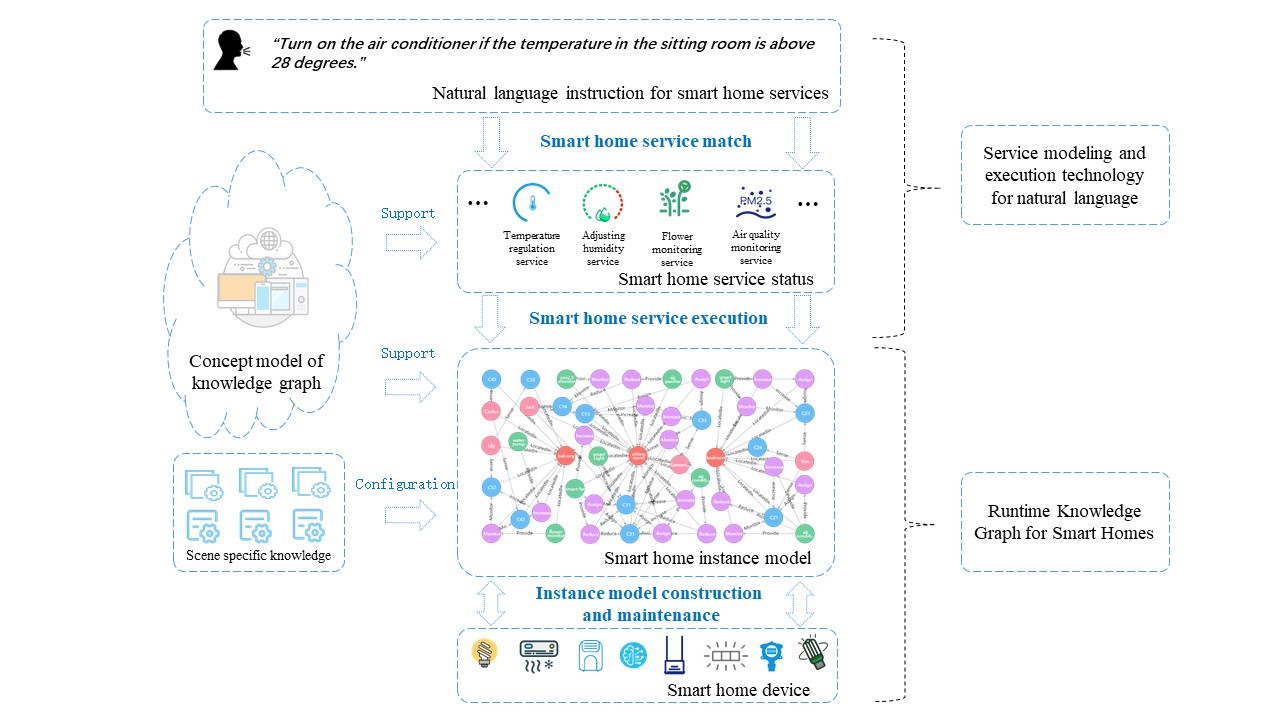
\includegraphics[width=0.9\textwidth]{overview.jpg}
	\caption{Overview of Supporting End-user Programming towards Smart Home Services}
	\label{fig:overview}
\end{figure}

Firstly, the runtime knowledge graph for smart home is proposed. This paper proposes a concept model of knowledge graph for context-aware services of smart home. Concept model of knowledge graph is a knowledge abstraction of the concept level of smart home situational awareness service, describe the concept and the relationship between the abstract elements in the scenario of smart home. The concept model defines the location, user, context, device, services and some concepts in the scenario of smart home. The concept model also defines the relationship such as located in, perception, provide, monitor, increase, reduce, etc. On this basis, the runtime construction method of smart home context-aware service knowledge graph instance model is proposed. The instance model represents smart home situational knowledge through concepts and relational instances, and describes the objective facts in specific scenes. Based on the runtime software architecture model of early work, the runtime construction methods of different types of concepts and relational cases are designed, and the two-way synchronization mechanism between the knowledge map instance model and specific smart home scenarios was established.

Secondly, service modeling and execution technology for natural language is proposed. The runtime knowledge graph for the built smart home generates the corresponding use case description for all the operations or rules on it. When the user sends natural language instructions, it matches the similarity degree with the use case description, so as to find the target operation or rules and automatically decide the device functions to be executed.

Based on the method above, the developer only need to declares the context-oriented knowledge of the scene, configures the mapping relationship between the concept instance and the smart device, and can map the natural language to the executable program on the runtime knowledge graph through the natural language service modeling, and finally formulates the final The service the user needs.

The user can quickly customize the smart home service according to the scene, and can wake up multiple similar devices in the same place to work together. For example, when the temperature needs to be adjusted, the method controls all the devices with temperature adjustment function in the room to meet the requirements of the user. The method can make simple decisions based on instructions from the user. Take an instructions sent by user for example. `Turn on the air conditioner if the temperature in the sitting room is above 28 degrees.' System can infer the information of the current use location based on the current location information of the user in the knowledge graph. The location information is `sitting room'. The system clarifies the instructions to `open the air conditioner in the living room', control the devices at the current location to provide services.

